% Copyright 2004 by Till Tantau <tantau@users.sourceforge.net>.
%
% In principle, this file can be redistributed and/or modified under
% the terms of the GNU Public License, version 2.
%
% However, this file is supposed to be a template to be modified
% for your own needs. For this reason, if you use this file as a
% template and not specifically distribute it as part of a another
% package/program, I grant the extra permission to freely copy and
% modify this file as you see fit and even to delete this copyright
% notice. 

\documentclass{beamer}
% There are many different themes available for Beamer. A comprehensive
% list with examples is given here:
% http://deic.uab.es/~iblanes/beamer_gallery/index_by_theme.html
% You can uncomment the themes below if you would like to use a different
% one:
%\usetheme{AnnArbor}
%\usetheme{Antibes}
%\usetheme{Bergen}
%\usetheme{Berkeley}
%\usetheme{Berlin}
\usetheme{Boadilla}
%\usetheme{boxes}
%\usetheme{CambridgeUS}
%\usetheme{Copenhagen}
%\usetheme{Darmstadt}
%\usetheme{default}
%\usetheme{Frankfurt}
%\usetheme{Goettingen}
%\usetheme{Hannover}
%\usetheme{Ilmenau}
%\usetheme{JuanLesPins}
%\usetheme{Luebeck}
%\usetheme{Madrid}
%\usetheme{Malmoe}
%\usetheme{Marburg}
%\usetheme{Montpellier}
%\usetheme{PaloAlto}
%\usetheme{Pittsburgh}
%\usetheme{Rochester}
%\usetheme{Singapore}
%\usetheme{Szeged}
%\usetheme{Warsaw}

\title{Assigning Boy Scouts to Patrols}

% A subtitle is optional and this may be deleted
%\subtitle{Optional Subtitle}

\author{Ian Bruce \and Julio Pineda \and Phil Snyder}

% We can cut the paper here

\date{MATH 480, Community Project}
% - Either use conference name or its abbreviation.
% - Not really informative to the audience, more for people (including
%   yourself) who are reading the slides online

\subject{Theoretical Computer Science}
% This is only inserted into the PDF information catalog. Can be left
% out. 

% If you have a file called "university-logo-filename.xxx", where xxx
% is a graphic format that can be processed by latex or pdflatex,
% resp., then you can add a logo as follows:x

% \pgfdeclareimage[height=0.5cm]{university-logo}{university-logo-filename}
% \logo{\pgfuseimage{university-logo}}

% Let's get started
\begin{document}

\begin{frame}
  \titlepage
\end{frame}

% Section and subsections will appear in the presentation overview
% and table of contents.
\begin{frame}{Problem Description}%{Optional Subtitle}
	\begin{itemize}
		\item Scoutmaster Gene Bruce of Troop 407 in Kent, Washington must assign new boy scouts into their patrols. In these patrols, the scouts engage in numerous activities and form close bonds. \\
		\vspace{0.2in}
		\item The number of incoming scouts are increasing, requiring multiple patrols to better organize activities and to form a small community between scouts.
		The younger scouts are temperamental and awkward when dealing with adversity, ruining their experience and causing many to quit. \\
		\vspace{0.2in}
		\item \textbf{Goal:  Assign 13 boy scouts of appropriate size (of 6-8 scouts) to two patrols such that we maximize the retention rate of the scouts by avoiding severe conflicts and maximizing positive relationships between scouts.}
	\end{itemize}
\end{frame}

\begin{frame}{Simplifications}
	\begin{itemize}
		\item Instead of considering the scouts' complex personality and their interactions with other scouts, we simplified by only asking each scout which other scouts they liked or disliked.
		\vspace{0.5in}
		\item Quality of the a patrol can be determined by the quality of the relationships between the unique pairs of the group. \\
		\textbf{i.e.} the whole is equal to the sum of its parts.
	\end{itemize}
\end{frame}

\begin{frame}{Acknowledgments}
	We would like to sincerely thank:
	\vspace{0.2in}
	\begin{itemize}
		\item \textbf{Scoutmaster Gene Bruce} for providing us the data and being extremely patient and understanding when discussing the background and problem.
		\vspace{0.2in}
		\item \textbf{Professor Sara Billey} for the mentorship and guidance throughout the entire project.
		\vspace{0.2in}
		\item \textbf{Austin Tran} for his helpful comments and suggestions.
	\end{itemize}
\end{frame}
% You can reveal the parts of a slide one at a time
% with the \pause command:
\begin{frame}{A Mathematical Interpretation - Let's Use Graphs!}
\begin{definition}
A \textbf{graph} consists of a group of objects called vertices where some of the vertices are linked together. When two vertices are linked, we say that there is an \textbf{edge} between them. 
\end{definition}
Implied by the name, graphs have a very visual interpretation, with the following being a typical example of what one would look like:
\begin{figure}
\centering
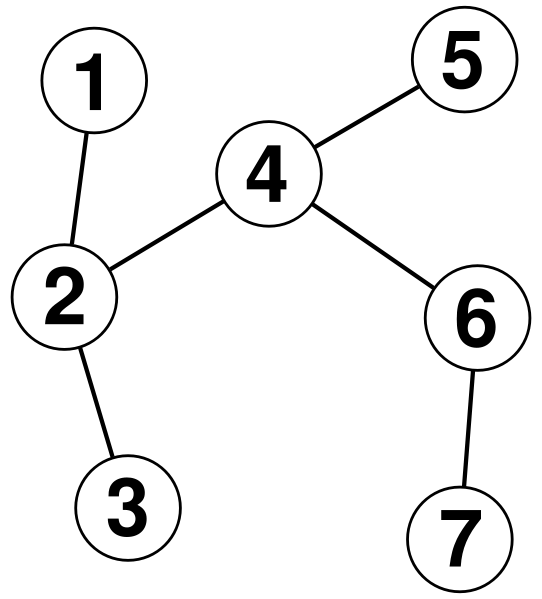
\includegraphics[scale=.1]{images/graph.png}
\end{figure}
The numbered circles represent vertices and the lines between them represent edges. We can model a wide variety of real-world things with graphs, namely any collection of objects where clear links can be drawn between pairs that share a relationship
\end{frame}

\begin{frame}{A Mathematical Interpretation cont.}
To give a mathematical structure to the patrol problem, we will use what is called a weighted directed graph:
\begin{definition}
A graph is \textbf{directed} if edges only represent one way relationships from one vertex to another
\end{definition}
\begin{definition}
A graph is \textbf{weighted} if a numerical value can be assigned to each edge
\end{definition}
With these definitions, we can define a graph where each scout is a vertex, and a directed edge from scout A to scout B is defined with weight 1 if scout A likes scout B, 0 if scout A is indifferent to B, and -1 if scout A dislikes scout B.
\end{frame}

\begin{frame}{A Mathematical Interpretation cont.}
\begin{itemize}
\item[]We have our graph, but how can we use it to divide the scouts into patrols? We can split up the vertices into groups that don't overlap, where this splitting is called a \textbf{partition}.
\item[]Each of these groups would correspond to a potential patrol.
\item[]We can imagine that there would be many different possible ways to split a graph, the key question is figure out which is "best" for the scouts.
\item[]If we could numerically measure the the "goodness" of a partition, we would want pick the partition that has maximal "goodness". Likewise, if we could numerically measure the the "badness" of a partition, we would want pick the partition that has minimal "badness". This is the essential method of how to \textbf{optimize} things mathematically.
\end{itemize}
\end{frame}

\begin{frame}{The Objective Functions}

\begin{enumerate}
\scriptsize
\item \textbf{MinCut}. This is the traditional metric of a cut on a weighted graph and is the sum of the weights of the edges we would ``cut'' if we were to sever the edges between distinct patrols. More formally, for some partition $I, J$ $I \neq J$, the MinCut is defined as:
$$
MinCut(I, J) := \sum_{e = (i, j), i \in I, j \in J}^{} c(e)
$$
We want this to be as low as possible.
\item \textbf{FriendCut}. This is the sum of the positive, or friendly edge weights within each patrol. That is, if $I_+ = \{e=(i,j) | i,j \in I, c(e)=1\}$ is the the set of edges in patrol $I$ with positive weight and $J_+ = \{e=(i,j) | i,j \in J, c(e)=1\}$ is the set of edges in patrol $J$ with positive weight, then (assuming all positive weights are 1):
$$
FriendCut(I, J) :=  |I_+ \cup J_+|
$$
We want this to be as high as possible.
\item \textbf{EnemyCut}. This is similar to FriendCut, except we now measure the number of negative edges going from one scout to another within the same patrol. Let $I_- = \{e=(i,j) | i,j \in I, c(e)=-1\}$ be the the set of edges in patrol $I$ with negative weight and $J_- = \{e=(i,j) | i,j \in J, c(e)=-1\}$ be the set of edges in patrol $J$ with negative weight, then
$$
EnemyCut(I, J) := |I_- \cup J_-|
$$
    We want this to be as low as possible.
\end{enumerate}
\end{frame}

\begin{frame}
\begin{enumerate}
    \scriptsize
        \setcounter{enumi}{3}
\item \textbf{AwkwardCut (+i)}. Same in all respects to MinCut, except for an additional penalty of $i$ if there are two scouts, Scout A and Scout B, in the same patrol such that Scout A likes Scout B and Scout B dislikes Scout A.
\begin{equation*}
    \begin{split}
        AwkwardCut&(I, J, i) := \Bigg[ \sum_{e = (k, j), k \in I, j \in J}^{} c(e) \Bigg] \\
        &+ i * \left\vert{\{e_+ = (k,j), e_- = (j, k) : e_+, e_- \in I, c(e_+) = 1, c(e_-) = -1\}}\right\vert
    \end{split}
\end{equation*}

\item \textbf{HybridCut}. A convex combination of MinCut and FriendCut, each with equal weight (that is, half the MinCut loss plus half the FriendCut loss).
\begin{equation*}
    HybridCut(I, J) := \frac{1}{2}MinCut(I, J) + \frac{1}{2}FriendCut(I, J)
\end{equation*}
\end{enumerate}
\end{frame}

\begin{frame}{Our Solution}

\begin{table}[h]
\centering
\footnotesize
\begin{tabular}{ |l|l|l|l|l|l| }
\hline
\multicolumn{2}{|c|}{\textbf{MinCut}} & \multicolumn{2}{|c|}{\textbf{FriendCut}} & \multicolumn{2}{|c|}{\textbf{EnemyCut}}\\
\hline
Patrol 1 & Patrol 2 & Patrol 1 & Patrol 2 & Patrol 1 & Patrol 2\\
\hline
Brandon & Christian & Brandon & Daniel & Brandon & Christian\\
Cameron & Daniel & Cameron & Darwin & Cameron & Jake\\
Colby & Jake & Christian & Jake & Colby & Jordan\\
Darwin & Jordan & Colby & Jordan  & Daniel & Nathan\\
Evan & Nathan & Evan & Nathan & Darwin & Patrick\\
Tommy & Patrick & Tommy & Patrick & Evan & Timmy\\
& Timmy & & Timmy & Tommy & \\
\hline
\multicolumn{6}{|c|}{\hphantom{1}} \\
\hline
\multicolumn{2}{|c|}{\textbf{AwkwardCut (+1)}} & \multicolumn{2}{|c|}{\textbf{AwkwardCut (+2)}} & \multicolumn{2}{|c|}{\textbf{HybridCut}} \\
\hline
Patrol 1 & Patrol 2 & Patrol 1 & Patrol 2 & Patrol 1 & Patrol 2\\
\hline
Brandon & Christian & Brandon & Cameron & Brandon & Christian\\
Cameron & Daniel & Christian & Evan & Cameron & Daniel\\
Colby & Jake & Daniel & Evan & Colby & Darwin\\
Darwin & Jordan & Darwin & Nathan & Evan & Jake\\
Evan & Nathan & Jake & Timmy & Timmy & Jordan\\
Tommy & Patrick & Jordan & Tommy & Tommy & Nathan\\
\hphantom{1} & Timmy & Patrick & \hphantom{1} & \hphantom{1} & Patrick\\
\hline
\end{tabular}
\caption{The partitions arrived at by minimizing each objective function}
\end{table}

\end{frame}

\begin{frame}{}
    \begin{block}{How Good Are These Solutions?}
\begin{figure}[h]
    \centering
    \begin{tabular}{ |l|l|l|l| }
        \hline
        \textbf{Method} & \textbf{MinCut} & \textbf{FriendCut} & \textbf{EnemyCut} \\
        \hline
        MinCut & 0 & 17 & 0 \\
        FriendCut & 1 & 18 & 1 \\
        EnemyCut & 2 & 15 & 0 \\
        AwkwardCut (+1) & 0 & 17 & 0 \\
        AwkwardCut (+2) & 1 & 18 & 2 \\
        HybridCut & 0 & 18 & 1 \\
        \hline
    \end{tabular}
    \caption{The scores according to the three primary metrics.}
\end{figure}
    \end{block}
\end{frame}

\begin{frame}{Blocks}
\begin{block}{Block Title}
You can also highlight sections of your presentation in a block, with it's own title
\end{block}
\begin{theorem}
There are separate environments for theorems, examples, definitions and proofs.
\end{theorem}
\begin{example}
Here is an example of an example block.
\end{example}
\end{frame}

% Placing a * after \section means it will not show in the
% outline or table of contents.
\section*{Summary}

\begin{frame}{Summary}
  \begin{itemize}
  \item
    The \alert{first main message} of your talk in one or two lines.
  \item
    The \alert{second main message} of your talk in one or two lines.
  \item
    Perhaps a \alert{third message}, but not more than that.
  \end{itemize}
  
  \begin{itemize}
  \item
    Outlook
    \begin{itemize}
    \item
      Something you haven't solved.
    \item
      Something else you haven't solved.
    \end{itemize}
  \end{itemize}
\end{frame}



% All of the following is optional and typically not needed. 
\appendix
\section<presentation>*{\appendixname}
\subsection<presentation>*{For Further Reading}

\begin{frame}[allowframebreaks]
  \frametitle<presentation>{For Further Reading}
    
  \begin{thebibliography}{10}
    
  \beamertemplatebookbibitems
  % Start with overview books.

  \bibitem{Author1990}
    A.~Author.
    \newblock {\em Handbook of Everything}.
    \newblock Some Press, 1990.
 
    
  \beamertemplatearticlebibitems
  % Followed by interesting articles. Keep the list short. 

  \bibitem{Someone2000}
    S.~Someone.
    \newblock On this and that.
    \newblock {\em Journal of This and That}, 2(1):50--100,
    2000.
  \end{thebibliography}
\end{frame}

\end{document}


